% Circumscribed Parallelepiped
% Author: Axel Pavillet
\documentclass[border=10pt]{standalone}
\usepackage{tkz-graph}
\usepackage{relsize}
\usepackage{adjustbox}
\usetikzlibrary{arrows,decorations.markings,calc}

\definecolor{cd40000}{RGB}{212,0,0}
\definecolor{cffffff}{RGB}{255,255,255}
\definecolor{c2a7fff}{RGB}{42,127,255}
\definecolor{c0000d9}{RGB}{0,0,217}
\definecolor{c0000ff}{RGB}{0,0,255}

\usepackage{relsize}

% \tikzset{every path/.style={draw, ->,>=latex,line width=1pt,color=black}}

%\tikzset{every node/.style={draw,minimum width = 20pt,line width = 1.75pt,
%circle,inner sep=0pt,font = \fontsize{14}{14}\selectfont,fill=none}}
\newcommand{\n}{\text{\raisebox{0.3ex}{-}}}

\begin{document}

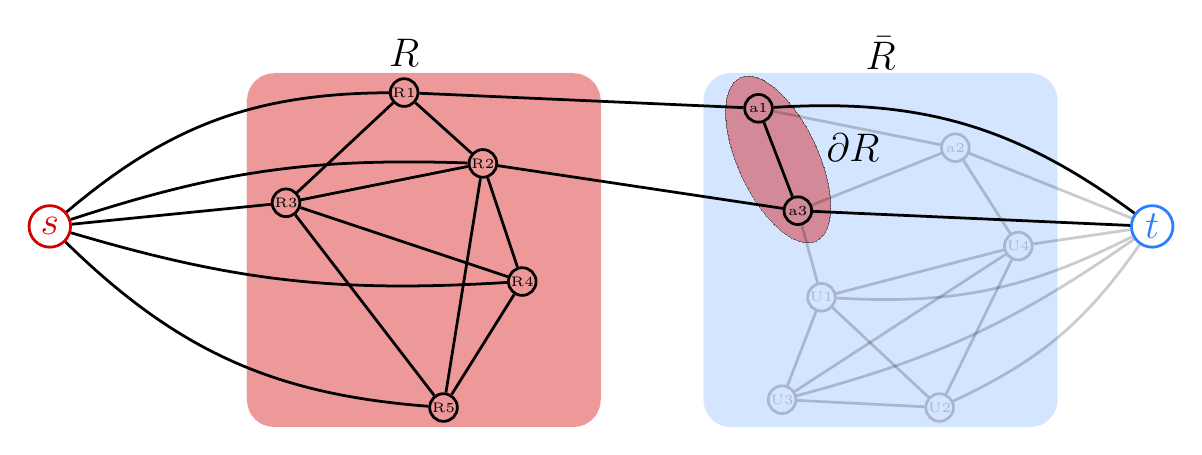
\begin{tikzpicture}[scale=1]

% \draw[color=black,line width=1pt] (0,0) rectangle ++(15,5);

\draw[color=white,rounded corners=10pt,line width=0pt,fill=cd40000, opacity=0.4] (3,-0.05) rectangle ++(4.5,4.5);

\draw[color=white,rounded corners=10pt,line width=0pt,fill=c2a7fff, opacity=0.2] (8.8,-0.05) rectangle ++(4.5,4.5);

%\draw [rotate around={-10:(10.95,3.85)}] (10.95,3.85) ellipse (0.7in and 0.2in);
\draw [rotate around={-65:(9.75,3.35)},line width=0pt,fill=cd40000,opacity=0.4] (9.75,3.35) ellipse (0.45in and 0.2in);

\begin{scope}[every node/.style={draw,minimum size=15,line width=1pt,circle,fill=none,font=\fontsize{14}{14}\selectfont,inner sep=0pt}]
\node[color=cd40000] (s) at (0.5,2.5) {$s$};
\node[color=c2a7fff] (t) at (14.5,2.5) {$t$};
\end{scope}


\begin{scope}[every node/.style={draw,minimum size=10,line width=1pt,circle,fill=none,font=\fontsize{5}{5}\selectfont,inner sep=0pt}]
\node (R1) at (5,4.2) {R1};
\node (R2) at (6,3.3) {R2};
\node (R3) at (3.5,2.8) {R3};
\node (R4) at (6.5,1.8) {R4};
\node (R5) at (5.5,0.2) {R5};
%\node (R6) at (3,1.5) {R6};
\node (aR1) at (9.5,4.0) {a1};
\node [opacity=0.2] (aR2) at (12,3.5) {a2};
\node (aR3) at (10,2.7) {a3};
\node [opacity=0.2] (U1) at (10.3,1.6) {U1};
\node [opacity=0.2] (U2) at (11.8,0.2) {U2};
\node [opacity=0.2] (U3) at (9.8,0.3) {U3};
\node [opacity=0.2] (U4) at (12.8,2.25) {U4};
\end{scope}
%
\begin{scope}[line width=1pt,color=black]
\draw[-] (R1) to (R2);
\draw[-] (R2) to (R4);
\draw[-] (R2) to (R5);
\draw[-] (R4) to (R5);
\draw[-] (R5) to (R3);
\draw[-] (R3) to (R1);
\draw[-] (R3) to (R4);
\draw[-] (R3) to (R2);
% \draw[-] (R6) to (R3);
% \draw[-] (R6) to (R4);
% \draw[-] (R6) to (R5);
\draw[-,opacity=0.2] (aR1) to (aR2);
\draw[-] (aR1) to (aR3);
\draw[-,opacity=0.2] (aR2) to (aR3);
\draw[-,opacity=0.2] (U1) to (U2);
\draw[-,opacity=0.2] (U1) to (U3);
\draw[-,opacity=0.2] (U1) to (U4);
\draw[-,opacity=0.2] (U2) to (U3);
\draw[-,opacity=0.2] (U2) to (U4);
\draw[-,opacity=0.2] (U3) to (U4);
\draw[-] (R1) to (aR1);
\draw[-] (R2) to (aR3);
\draw[-,opacity=0.2] (aR2) to (U4);
\draw[-,opacity=0.2] (aR3) to (U1);
\end{scope}

%
\begin{scope}[line width=1pt]
\draw[-] (s) to [bend left=20] (R1);
\draw[-] (s) to [bend left=10] (R2);
\draw[-] (s) to [bend right=0] (R3);
\draw[-] (s) to [bend right=10] (R4);
\draw[-] (s) to [bend right=20] (R5);
\end{scope}

\begin{scope}[line width=1pt]
\draw[-] (aR1) to [bend left=20] (t);
\draw[-,opacity=0.2] (aR2) to [bend left=0] (t);
\draw[-] (aR3) to [bend right=0] (t);
\end{scope}

\begin{scope}[line width=1pt]
\draw[-,opacity=0.2] (U1) to [bend right=15] (t);
\draw[-,opacity=0.2] (U2) to [bend right=15] (t);
\draw[-,opacity=0.2] (U3) to [bend right=10] (t);
\draw[-,opacity=0.2] (U4) to [bend left=0] (t);
\end{scope}

% \draw[color=cd40000,rounded corners=10pt,line width=2pt,dashed] (2.25,-0.8) rectangle ++(4.75,10);
% \draw[color=c2a7fff,rounded corners=10pt,line width=2pt,dashed] (8,-0.8) rectangle ++(4.75,10);
% \draw[color=yellow,rounded corners=10pt,line width=2pt,dashed] (8.25,4.5) rectangle ++(4.25,4.25);

\node[line width=0,font=\fontsize{14}{14}\selectfont] at (5,4.7) {$R$};
\node[line width=0,font=\fontsize{14}{14}\selectfont] at (11.05,4.7) {$\bar{R}$};
\node[line width=0,font=\fontsize{14}{14}\selectfont] at (10.7,3.5) {$\partial R$};

\end{tikzpicture}

\end{document}
